\documentclass[a4paper,11pt]{beamer}

\usepackage{préambule}

\begin{document}

\begin{center}
	\begin{frame}
		\begin{center}
			\LARGE
			\uline{Exercices : symétrie axiale}
			\vspace{1em}
		\end{center}
	\end{frame}

	\begin{frame}
		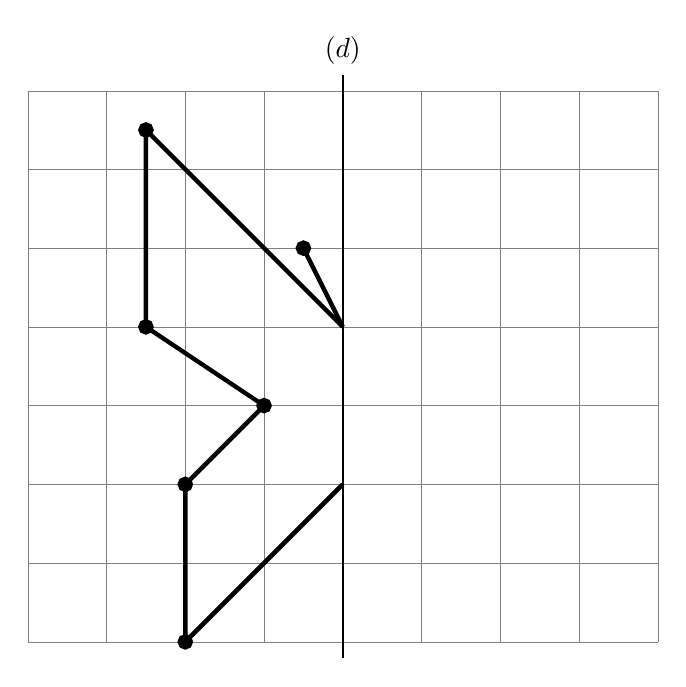
\begin{tikzpicture}[scale=1,c/.style={insert path={circle[radius=2pt]},fill}]
			\draw[gray,ultra thin] (0,0) grid (8,7);
			\draw[black,thick] (4,-0.2) -- (4,7.2) node[anchor=south]{$(d)$};

			\draw[black,ultra thick]
			(4,4)
			-- ++(-2.5,2.5) [c]
			-- ++(0,-2.5) [c]
			-- ++(1.5,-1) [c]
			-- ++(-1,-1) [c]
			-- ++(0,-2) [c]
			-- ++(2,2);
			\draw[black,ultra thick] (4,4) -- ++(-0.5,1) [c];
		\end{tikzpicture}
	\end{frame}

	\begin{frame}
		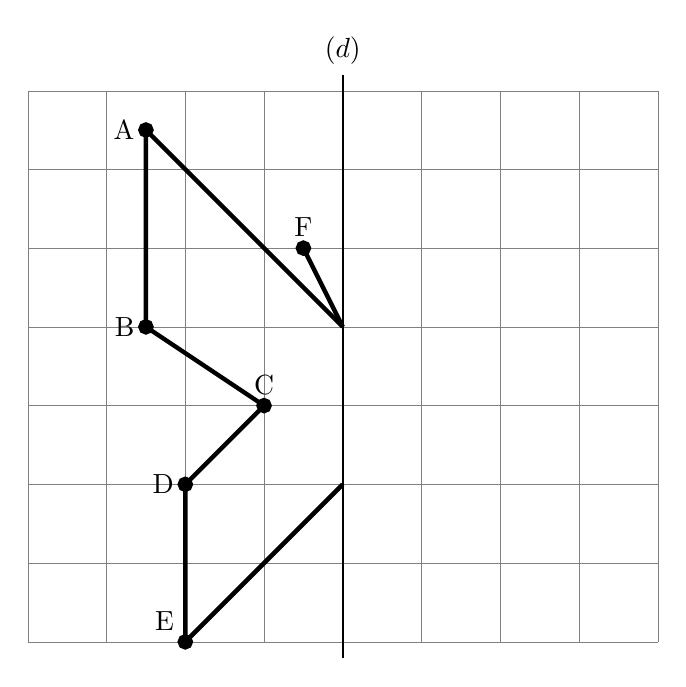
\begin{tikzpicture}[scale=1,c/.style={insert path={circle[radius=2pt]},fill}]
			\draw[gray,ultra thin] (0,0) grid (8,7);
			\draw[black,thick] (4,-0.2) -- (4,7.2) node[anchor=south]{$(d)$};

			\draw[black,ultra thick]
			(4,4)
			-- ++(-2.5,2.5) [c] node[anchor=east] {A}
			-- ++(0,-2.5) [c] node[anchor=east] {B}
			-- ++(1.5,-1) [c] node[anchor=south] {C}
			-- ++(-1,-1) [c] node[anchor=east] {D}
			-- ++(0,-2) [c] node[anchor=south east] {E}
			-- ++(2,2);
			\draw[black,ultra thick] (4,4) -- ++(-0.5,1) [c] node[anchor=south] {F};
		\end{tikzpicture}
	\end{frame}

	\begin{frame}
		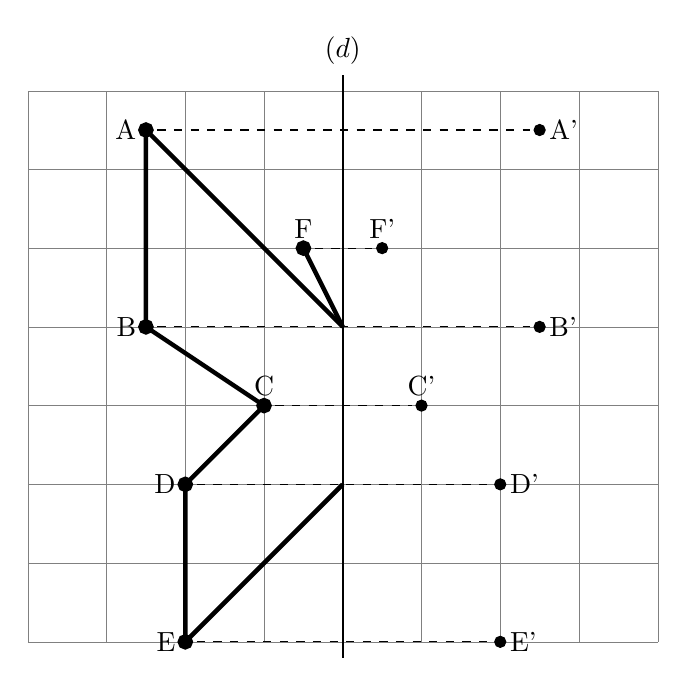
\begin{tikzpicture}[scale=1,c/.style={insert path={circle[radius=2pt]},fill}]
			\draw[gray,ultra thin] (0,0) grid (8,7);
			\draw[black,thick] (4,-0.2) -- (4,7.2) node[anchor=south]{$(d)$};

			\draw[black,ultra thick]
			(4,4)
			-- ++(-2.5,2.5) [c] node (A) {}
			-- ++(0,-2.5) [c] node (B) {}
			-- ++(1.5,-1) [c] node (C) {}
			-- ++(-1,-1) [c] node (D) {}
			-- ++(0,-2) [c] node (E) {}
			-- ++(2,2);
			\draw[black,ultra thick] (4,4) -- ++(-0.5,1) [c] node (F) {};

			\draw
			(4,4)
			++(2.5,2.5) [c] node (A') {}
			++(0,-2.5) [c] node (B') {}
			++(-1.5,-1) [c] node (C') {}
			++(1,-1) [c] node (D') {}
			++(0,-2) [c] node (E') {}
			++(-2,2);
			\draw (4,4) ++(0.5,1) [c] node (F') {};

			\node[right] at (A') {A'};
			\node[right] at (B') {B'};
			\node[above] at (C') {C'};
			\node[right] at (D') {D'};
			\node[right] at (E') {E'};
			\node[above] at (F') {F'};
			\node[left] at (A) {A};
			\node[left] at (B) {B};
			\node[above] at (C) {C};
			\node[left] at (D) {D};
			\node[left] at (E) {E};
			\node[above] at (F) {F};
			\draw[dashed] (A) -- (A');
			\draw[dashed] (B) -- (B');
			\draw[dashed] (C) -- (C');
			\draw[dashed] (D) -- (D');
			\draw[dashed] (E) -- (E');
			\draw[dashed] (F) -- (F');
		\end{tikzpicture}
	\end{frame}

	\begin{frame}
		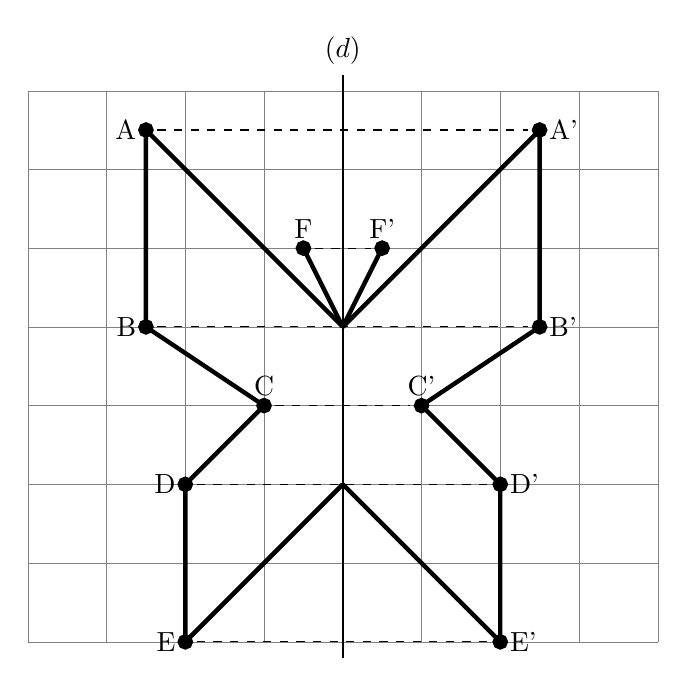
\begin{tikzpicture}[scale=1,c/.style={insert path={circle[radius=2pt]},fill}]
			\draw[gray,ultra thin] (0,0) grid (8,7);
			\draw[black,thick] (4,-0.2) -- (4,7.2) node[anchor=south]{$(d)$};

			\draw[black,ultra thick]
			(4,4)
			-- ++(-2.5,2.5) [c] node (A) {}
			-- ++(0,-2.5) [c] node (B) {}
			-- ++(1.5,-1) [c] node (C) {}
			-- ++(-1,-1) [c] node (D) {}
			-- ++(0,-2) [c] node (E) {}
			-- ++(2,2);
			\draw[black,ultra thick] (4,4) -- ++(-0.5,1) [c] node (F) {};

			\draw[black,ultra thick]
			(4,4)
			-- ++(2.5,2.5) [c] node (A') {}
			-- ++(0,-2.5) [c] node (B') {}
			-- ++(-1.5,-1) [c] node (C') {}
			-- ++(1,-1) [c] node (D') {}
			-- ++(0,-2) [c] node (E') {}
			-- ++(-2,2);
			\draw[black,ultra thick] (4,4) -- ++(0.5,1) [c] node (F') {};

			\node[right] at (A') {A'};
			\node[right] at (B') {B'};
			\node[above] at (C') {C'};
			\node[right] at (D') {D'};
			\node[right] at (E') {E'};
			\node[above] at (F') {F'};
			\node[left] at (A) {A};
			\node[left] at (B) {B};
			\node[above] at (C) {C};
			\node[left] at (D) {D};
			\node[left] at (E) {E};
			\node[above] at (F) {F};
			\draw[dashed] (A) -- (A');
			\draw[dashed] (B) -- (B');
			\draw[dashed] (C) -- (C');
			\draw[dashed] (D) -- (D');
			\draw[dashed] (E) -- (E');
			\draw[dashed] (F) -- (F');
		\end{tikzpicture}

		On obtient un papillon.
	\end{frame}

	\begin{frame}
		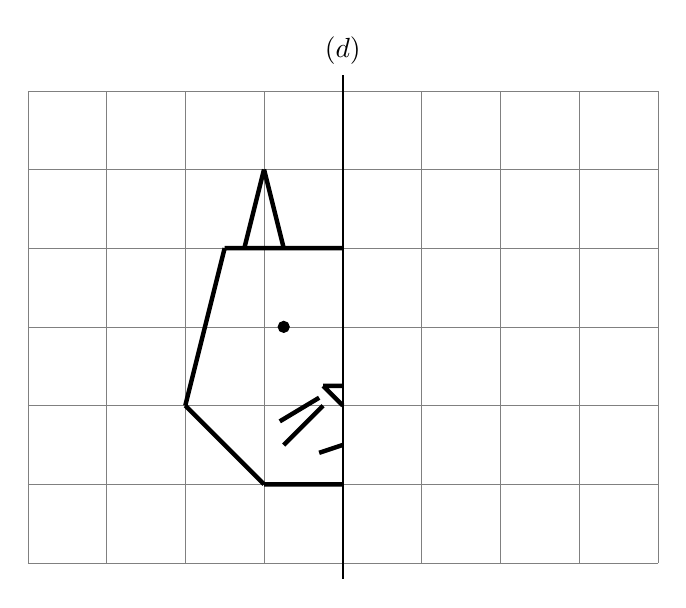
\begin{tikzpicture}[c/.style={insert path={circle[radius=0pt]},fill}]
			\draw[gray,ultra thin] (0,0) grid (8,6);
			\draw[black,thick] (4,-0.2) -- (4,6.2) node[anchor=south]{$(d)$};

			% head
			\draw[black,ultra thick] (4,1) -- ++(-1,0) [c] -- ++(-1,1) [c] -- ++(0.5,2) [c] -- ++(1.5,0);
			% ear
			\draw[black,ultra thick] (3.25,4) [c] -- ++(-0.25,1) [c] -- ++(-0.25,-1) [c];
			% nose
			\draw[black,ultra thick] (4,2) -- ++(-0.25,0.25) [c] -- ++(0.25,0);
			% eye
			\draw[black,fill] (3.25,3) circle (2pt);
			% mustache
			\draw[black,ultra thick] (3.75,2) -- ++(-0.5,-0.5);
			\draw[black,ultra thick] (3.7,2.1) -- ++(-0.5,-0.3);
			% mouth
			\draw[black,ultra thick] (4,1.5) -- ++(-0.3,-0.1);
		\end{tikzpicture}
	\end{frame}

	\begin{frame}
		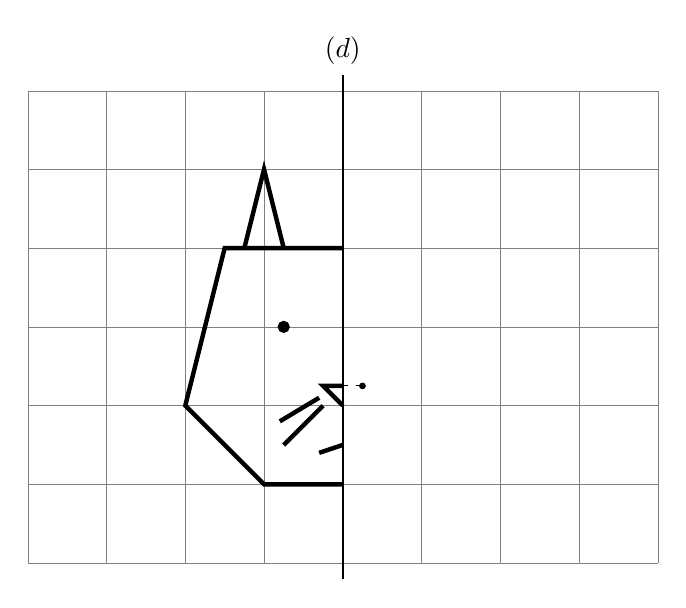
\begin{tikzpicture}[c/.style={insert path={circle[radius=1pt]},fill}]
			\draw[gray,ultra thin] (0,0) grid (8,6);
			\draw[black,thick] (4,-0.2) -- (4,6.2) node[anchor=south]{$(d)$};

			% head
			\draw[black,ultra thick] (4,1) -- ++(-1,0) -- ++(-1,1) -- ++(0.5,2) -- ++(1.5,0);
			% ear
			\draw[black,ultra thick] (3.25,4) -- ++(-0.25,1) -- ++(-0.25,-1);
			% nose
			\draw[black,ultra thick] (4,2) -- ++(-0.25,0.25) -- ++(0.25,0);
			% eye
			\draw[black,fill] (3.25,3) circle (2pt);
			% mustache
			\draw[black,ultra thick] (3.75,2) -- ++(-0.5,-0.5);
			\draw[black,ultra thick] (3.7,2.1) -- ++(-0.5,-0.3);
			% mouth
			\draw[black,ultra thick] (4,1.5) -- ++(-0.3,-0.1);

			\draw (4,2) ++(0.25,0.25) [c] ++(-0.25,0);

			\draw[dashed] (3.75,2.25) -- (4.25,2.25);
		\end{tikzpicture}
	\end{frame}

	\begin{frame}
		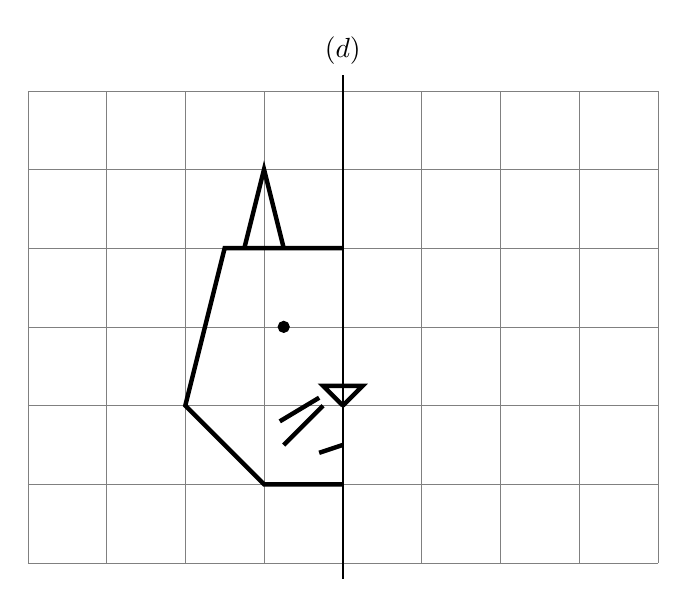
\begin{tikzpicture}[c/.style={insert path={circle[radius=1pt]},fill}]
			\draw[gray,ultra thin] (0,0) grid (8,6);
			\draw[black,thick] (4,-0.2) -- (4,6.2) node[anchor=south]{$(d)$};

			% head
			\draw[black,ultra thick] (4,1) -- ++(-1,0) -- ++(-1,1) -- ++(0.5,2) -- ++(1.5,0);
			% ear
			\draw[black,ultra thick] (3.25,4) -- ++(-0.25,1) -- ++(-0.25,-1);
			% nose
			\draw[black,ultra thick] (4,2) -- ++(-0.25,0.25) -- ++(0.25,0);
			% eye
			\draw[black,fill] (3.25,3) circle (2pt);
			% mustache
			\draw[black,ultra thick] (3.75,2) -- ++(-0.5,-0.5);
			\draw[black,ultra thick] (3.7,2.1) -- ++(-0.5,-0.3);
			% mouth
			\draw[black,ultra thick] (4,1.5) -- ++(-0.3,-0.1);

			\draw[black,ultra thick] (4,2) -- ++(0.25,0.25) -- ++(-0.25,0);
		\end{tikzpicture}
	\end{frame}

	\begin{frame}
		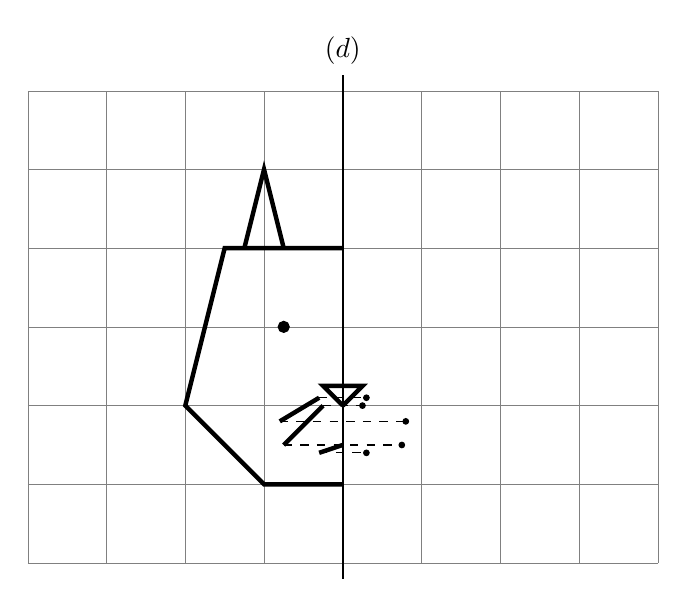
\begin{tikzpicture}[c/.style={insert path={circle[radius=1pt]},fill}]
			\draw[gray,ultra thin] (0,0) grid (8,6);
			\draw[black,thick] (4,-0.2) -- (4,6.2) node[anchor=south]{$(d)$};

			% head
			\draw[black,ultra thick] (4,1) -- ++(-1,0) -- ++(-1,1) -- ++(0.5,2) -- ++(1.5,0);
			% ear
			\draw[black,ultra thick] (3.25,4) -- ++(-0.25,1) -- ++(-0.25,-1);
			% nose
			\draw[black,ultra thick] (4,2) -- ++(-0.25,0.25) -- ++(0.25,0);
			% eye
			\draw[black,fill] (3.25,3) circle (2pt);
			% mustache
			\draw[black,ultra thick] (3.75,2) -- ++(-0.5,-0.5);
			\draw[black,ultra thick] (3.7,2.1) -- ++(-0.5,-0.3);
			% mouth
			\draw[black,ultra thick] (4,1.5) -- ++(-0.3,-0.1);

			\draw[black,ultra thick] (4,2) -- ++(0.25,0.25) -- ++(-0.25,0);
			\draw (4.25,2) [c] ++(0.5,-0.5) [c];
			\draw (4.3,2.1) [c] ++(0.5,-0.3) [c];
			\draw (4,1.5) ++(0.3,-0.1) [c];

			\draw[dashed] (3.75,2) -- (4.25,2);
			\draw[dashed] (3.7,2.1) -- (4.3,2.1);
			\draw[dashed] (3.25,1.5) -- (4.75,1.5);
			\draw[dashed] (3.2,1.8) -- (4.8,1.8);
			\draw[dashed] (3.7,1.4) -- (4.3,1.4);
		\end{tikzpicture}
	\end{frame}

	\begin{frame}
		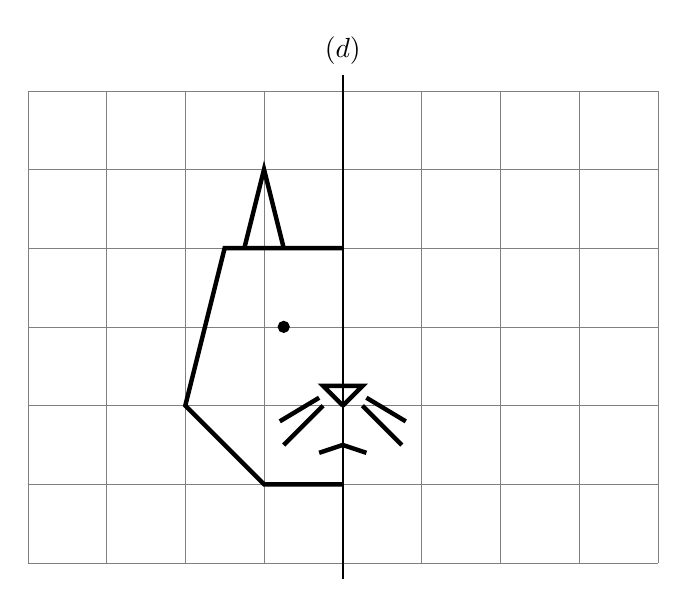
\begin{tikzpicture}[c/.style={insert path={circle[radius=1pt]},fill}]
			\draw[gray,ultra thin] (0,0) grid (8,6);
			\draw[black,thick] (4,-0.2) -- (4,6.2) node[anchor=south]{$(d)$};

			% head
			\draw[black,ultra thick] (4,1) -- ++(-1,0) -- ++(-1,1) -- ++(0.5,2) -- ++(1.5,0);
			% ear
			\draw[black,ultra thick] (3.25,4) -- ++(-0.25,1) -- ++(-0.25,-1);
			% nose
			\draw[black,ultra thick] (4,2) -- ++(-0.25,0.25) -- ++(0.25,0);
			% eye
			\draw[black,fill] (3.25,3) circle (2pt);
			% mustache
			\draw[black,ultra thick] (3.75,2) -- ++(-0.5,-0.5);
			\draw[black,ultra thick] (3.7,2.1) -- ++(-0.5,-0.3);
			% mouth
			\draw[black,ultra thick] (4,1.5) -- ++(-0.3,-0.1);

			\draw[black,ultra thick] (4,2) -- ++(0.25,0.25) -- ++(-0.25,0);
			\draw[black,ultra thick] (4.25,2) -- ++(0.5,-0.5);
			\draw[black,ultra thick] (4.3,2.1) -- ++(0.5,-0.3);
			\draw[black,ultra thick] (4,1.5) -- ++(0.3,-0.1);
		\end{tikzpicture}
	\end{frame}

	\begin{frame}
		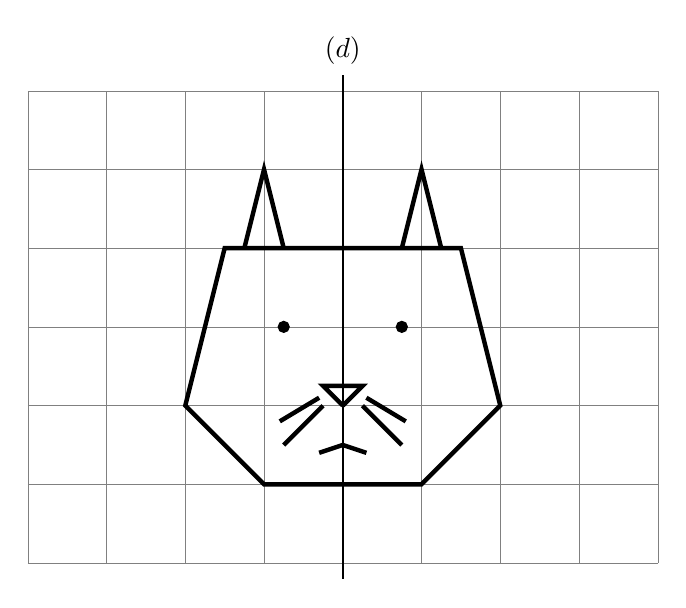
\begin{tikzpicture}[c/.style={insert path={circle[radius=1pt]},fill}]
			\draw[gray,ultra thin] (0,0) grid (8,6);
			\draw[black,thick] (4,-0.2) -- (4,6.2) node[anchor=south]{$(d)$};

			% head
			\draw[black,ultra thick] (4,1) -- ++(-1,0) -- ++(-1,1) -- ++(0.5,2) -- ++(1.5,0);
			% ear
			\draw[black,ultra thick] (3.25,4) -- ++(-0.25,1) -- ++(-0.25,-1);
			% nose
			\draw[black,ultra thick] (4,2) -- ++(-0.25,0.25) -- ++(0.25,0);
			% eye
			\draw[black,fill] (3.25,3) circle (2pt);
			% mustache
			\draw[black,ultra thick] (3.75,2) -- ++(-0.5,-0.5);
			\draw[black,ultra thick] (3.7,2.1) -- ++(-0.5,-0.3);
			% mouth
			\draw[black,ultra thick] (4,1.5) -- ++(-0.3,-0.1);

			% head
			\draw[black,ultra thick] (4,1) -- ++(1,0) -- ++(1,1) -- ++(-0.5,2) -- ++(-1.5,0);
			% ear
			\draw[black,ultra thick] (4.75,4) -- ++(0.25,1) -- ++(0.25,-1);
			% nose
			\draw[black,ultra thick] (4,2) -- ++(0.25,0.25) -- ++(-0.25,0);
			% eye
			\draw[black,fill] (4.75,3) circle (2pt);
			% mustache
			\draw[black,ultra thick] (4.25,2) -- ++(0.5,-0.5);
			\draw[black,ultra thick] (4.3,2.1) -- ++(0.5,-0.3);
			% mouth
			\draw[black,ultra thick] (4,1.5) -- ++(0.3,-0.1);
		\end{tikzpicture}

		On obtient un chat.
	\end{frame}

	\newcommand{\sqrttwo}{\directlua{tex.print(math.sqrt(2))}}
	\newcommand{\timessqrttwo}[1]{\directlua{tex.print(math.sqrt(2) * tonumber(#1))}}

	\begin{frame}
		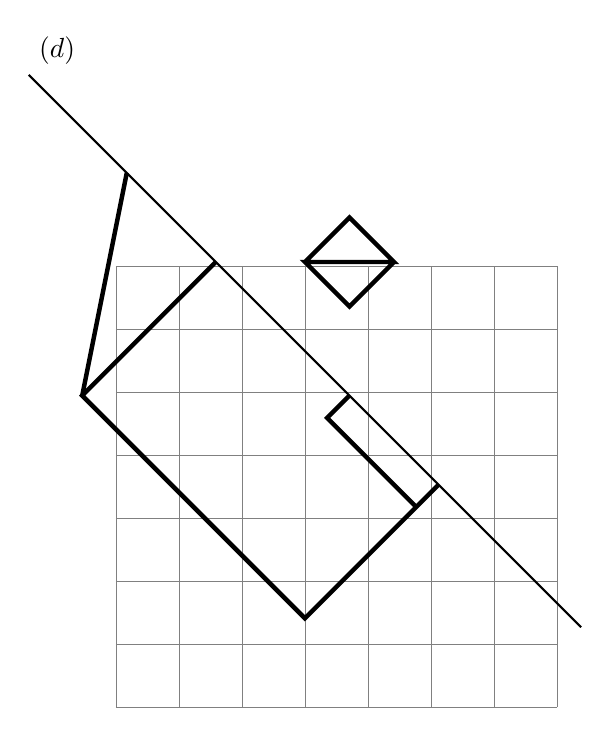
\begin{tikzpicture}[scale=0.8,c/.style={insert path={circle[radius=1pt]},fill}]
			\draw[step=\sqrttwo,gray,ultra thin] (\timessqrttwo{-3},\timessqrttwo{0}) grid ++(\timessqrttwo{7},\timessqrttwo{7});
			\draw[black,thick,rotate=45] (4,-2.2) -- (4,10.2) node[anchor=south west]{$(d)$};

			\draw[black,ultra thick,rotate=45] (4,1) -- ++(-3,0) -- ++(0,5) -- ++(3,0);
			\draw[black,ultra thick,rotate=45] (4,8) -- ++(-3,-2);
			\draw[black,ultra thick,rotate=45] (3.5,1) -- ++(0,2) -- ++(0.5,0);
			\draw[black,ultra thick,rotate=45] (6,4) -- ++(-1,0) -- ++(0,1) -- ++(1,-1) -- ++(0,1) -- ++(-1,0);
		\end{tikzpicture}
	\end{frame}

	\begin{frame}
		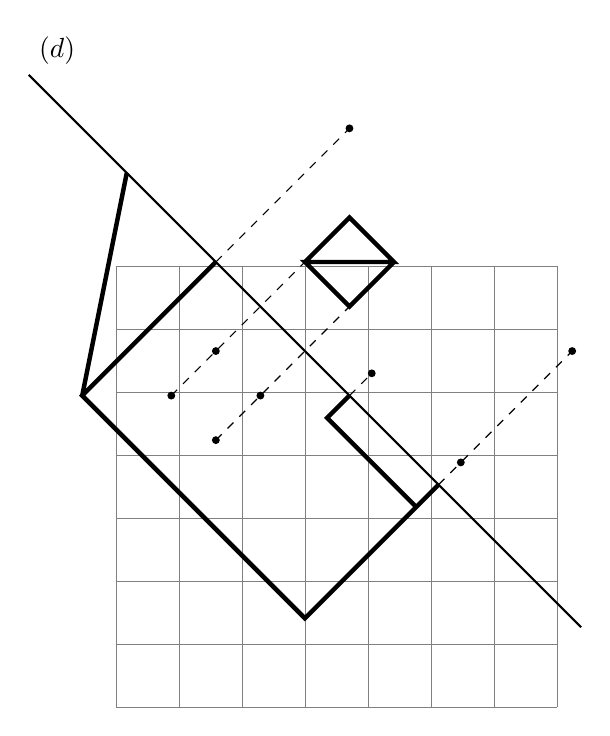
\begin{tikzpicture}[scale=0.8,c/.style={insert path={circle[radius=1.5pt]},fill}]
			\draw[step=\sqrttwo,gray,ultra thin] (\timessqrttwo{-3},\timessqrttwo{0}) grid ++(\timessqrttwo{7},\timessqrttwo{7});
			\draw[black,thick,rotate=45] (4,-2.2) -- (4,10.2) node[anchor=south west]{$(d)$};

			\draw[black,ultra thick,rotate=45] (4,1) -- ++(-3,0) -- ++(0,5) -- ++(3,0);
			\draw[black,ultra thick,rotate=45] (4,8) -- ++(-3,-2);
			\draw[black,ultra thick,rotate=45] (3.5,1) -- ++(0,2) -- ++(0.5,0);
			\draw[black,ultra thick,rotate=45] (6,4) -- ++(-1,0) -- ++(0,1) -- ++(1,-1) -- ++(0,1) -- ++(-1,0);

			\draw[rotate=45] (4,1) ++(3,0) [c] ++(0,5) [c] ++(-3,0);
			\draw[rotate=45] (4,8) ++(3,-2);
			\draw[rotate=45] (4.5,1) [c] ++(0,2) [c] ++(-0.5,0);
			\draw[rotate=45] (2,4) [c] ++(1,0) [c] ++(0,1) [c] ++(-1,-1) ++(0,1) [c] ++(1,0);

			\draw[dashed,rotate=45] (2,4) -- (6,4);
			\draw[dashed,rotate=45] (2,5) -- (6,5);
			\draw[dashed,rotate=45] (4,6) -- (7,6);
			\draw[dashed,rotate=45] (4,3) -- (4.5,3);
			\draw[dashed,rotate=45] (4,1) -- (7,1);
		\end{tikzpicture}
	\end{frame}

	\begin{frame}
		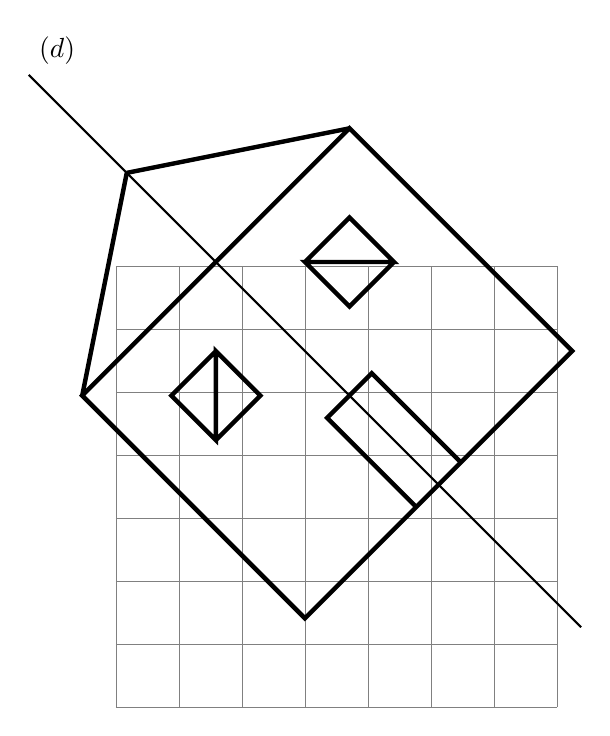
\begin{tikzpicture}[scale=0.8,c/.style={insert path={circle[radius=1.5pt]},fill}]
			\draw[step=\sqrttwo,gray,ultra thin] (\timessqrttwo{-3},\timessqrttwo{0}) grid ++(\timessqrttwo{7},\timessqrttwo{7});
			\draw[black,thick,rotate=45] (4,-2.2) -- (4,10.2) node[anchor=south west]{$(d)$};

			\draw[black,ultra thick,rotate=45] (4,1) -- ++(-3,0) -- ++(0,5) -- ++(3,0);
			\draw[black,ultra thick,rotate=45] (4,8) -- ++(-3,-2);
			\draw[black,ultra thick,rotate=45] (3.5,1) -- ++(0,2) -- ++(0.5,0);
			\draw[black,ultra thick,rotate=45] (6,4) -- ++(-1,0) -- ++(0,1) -- ++(1,-1) -- ++(0,1) -- ++(-1,0);

			\draw[black,ultra thick,rotate=45] (4,1) -- ++(3,0) -- ++(0,5) -- ++(-3,0);
			\draw[black,ultra thick,rotate=45] (4,8) -- ++(3,-2);
			\draw[black,ultra thick,rotate=45] (4.5,1) -- ++(0,2) -- ++(-0.5,0);
			\draw[black,ultra thick,rotate=45] (2,4) -- ++(1,0) -- ++(0,1) -- ++(-1,-1) -- ++(0,1) -- ++(1,0);
		\end{tikzpicture}

		On obtient une maison.
	\end{frame}
\end{center}

\end{document}